\documentclass{article}
\usepackage{fancyhdr}
\usepackage{ctex}
\usepackage{listings}
\usepackage[a4paper, body={18cm,22cm}]{geometry}
\usepackage{amsmath,amssymb,amstext,wasysym,enumerate,graphicx}
\usepackage{float,abstract,booktabs,indentfirst,amsmath}
\usepackage{multirow}
\usepackage{enumitem}
\usepackage{listings}
\usepackage{xcolor}
\usepackage{tabularx}
\usepackage{subfigure}
\usepackage[most]{tcolorbox}
\usepackage{accsupp}
\usepackage[backend=biber,style=numeric]{biblatex}
\usepackage[xetex]{hyperref}
\usetikzlibrary{arrows.meta}
\newcommand\emptyaccsupp[1]{\BeginAccSupp{ActualText={}}#1\EndAccSupp{}}
\setlength{\parindent}{2em}
\renewcommand\arraystretch{1.4}
% \setmonofont{FiraCode Nerd Font}
\setCJKmonofont{黑体}
% \setmainfont{Times New Roman}
% \hypersetup{CJKbookmarks=true,colorlinks=true,citecolor=blue,%
%             linkcolor=blue,urlcolor=blue,bookmarksnumbered=true,%
%             bookmarksopen=true,breaklinks=true}
\lstset{
    % language = C,
    xleftmargin = 3em,xrightmargin = 3em, aboveskip = 1em,
	backgroundcolor = \color{white}, % 背景色
	basicstyle = \small\ttfamily, % 基本样式 + 小号字体
	rulesepcolor= \color{gray}, % 代码块边框颜色
	breaklines = true, % 代码过长则换行
	numbers = left, % 行号在左侧显示
	numberstyle = \small\emptyaccsupp, % 行号字体
    numbersep = -14pt, 
    keywordstyle=\color{purple}\bfseries, % 关键字颜色
    commentstyle =\color{red!50!green!50!blue!60}, % 注释颜色
    stringstyle = \color{red}, % 字符串颜色
    morekeywords={ASSERT, int64_t, uint32_t},
	frame = shadowbox, % 用(带影子效果)方框框住代码块
	showspaces = false, % 不显示空格
    showstringspaces = false,
	columns = fixed, % 字间距固定
    literate=
        {^+}{{{\color{black}\textbf{+}}\colorbox{green!30}{\phantom{XX}}}}1
        {+\t}{{{\color{black}\textbf{+}}\colorbox{green!30}{\phantom{XX}}}}1,
}

%%%%%%%%%%%%%%%%%%%%%%%%%%%%%%%%%%%%%%%%%%%%%%%%%%%%
\addbibresource{references.bib}
%%%%%%%%%%%%%%%%%%%%%%%%%%%%%%%%%%%%%%%%%%%%%%%%%%%%

%%%%%%%%%%%%%%%%%%%%%%%%%%%%%%%%%%%%%%%%%%%%%%%%%%%%
% contstants
\newcommand{\course}{《智能计算系统》课程期中项目}
\newcommand{\titleText}{图像风格迁移}
\newcommand{\authorName}{李鹏达}
\newcommand{\authorID}{10225101460}
\newcommand{\yearMonth}{2025年5月}
%%%%%%%%%%%%%%%%%%%%%%%%%%%%%%%%%%%%%%%%%%%%%%%%%%%%

\title{\titleText}
\author{\authorName}

% 页眉页脚设置
\pagestyle{fancy}
\fancyhf{}
\fancyhead[L]{\course}
\fancyhead[R]{\titleText}
\fancyfoot[C]{\thepage}

\begin{document}

% title
\begin{titlepage}
    \title{\titleText}
    \author{\authorName}
    \thispagestyle{fancy}
    \fancyfoot{}
    \begin{center}
        \phantom{ }
        \vspace{5cm}
        \\
        
\includegraphics[width=0.9\textwidth]{img/ecnu.png}
        \vspace{1cm}
        \\
        \textbf{\fontsize{22}{36}\selectfont{\heiti \course}} 
        \vspace{2cm}
        \\
        \textbf{\fontsize{20}{26}\selectfont{\titleText}}  
        \vspace{2cm}
        \\
        \large
        \begin{tabular}{cp{4cm}<{\centering}}
            姓\quad 名:& \authorName \\
            \cline{2-2} \\[-2em]
            学\quad 号:& \authorID \\
            \cline{2-2} \\
        \end{tabular}
        \vspace{2cm}
        \\
        \large \yearMonth
    \end{center}
\end{titlepage}

\pagenumbering{arabic}
\setcounter{page}{1}

\section{实验背景}

图像风格迁移是一项旨在将一幅图像的内容结构与另一幅图像的艺术风格相结合的计算机视觉任务。传统方法主要依赖于图像处理技术与纹理合成算法,例如基于非参数采样的纹理合成方法\cite{efros1999texture},但这类方法在内容与风格的有效分离方面存在较大局限,生成图像的表达能力有限。

随着深度学习技术的迅速发展,Gatys 等人于 2015 年首次提出了基于卷积神经网络的图像风格迁移方法\cite{gatys2015neural},并取得了显著突破。这一方法首次实现了基于神经网络的、具有高质量视觉效果的图像风格迁移,并开启了后续多种风格迁移技术的发展,为本实验提供了理论基础和技术支撑。

\section{实验内容}

\subsection{所选神经网络模型简介}

Gatys 等人风格迁移方法\cite{gatys2015neural}通过对输出图像进行迭代优化,在风格迁移质量上取得了显著成果,但其每处理一张图像需数百次迭代,计算效率极低,难以满足实时应用需求。为此,Johnson 等人于 2016 年提出了 \emph{Fast Style Transfer} 模型 \cite{johnson2016perceptual},采用前馈卷积神经网络进行图像变换,并通过感知损失(Perceptual Loss)进行训练,实现了高质量且近实时的风格迁移。在实验中,我们将基于该模型进行实现。

\subsubsection{网络结构}

该方法的核心是训练一个图像变换网络 $f_W(x)$,将输入的内容图像 $x$ 映射为风格化输出图像 $\hat{y} = f_W(x)$。

图 \ref{fig:network} 展示了网络的基本结构,输入图像 $x$ 首先通过图像变换网络 $f_W$ 生成合成图像 $\hat{y}$。为了确保 $\hat{y}$ 在内容上接近内容目标图像 $y_c$,并在风格上与风格目标图像 $y_s$ 匹配,利用预训练的 VGG-16 网络 \cite{simonyan2014very} $\phi$ 作为损失网络。内容损失通过比较 $\hat{y}$ 和 $y_c$ 在 $\phi$ 的 \texttt{relu3\_3} 层的特征表示计算得到;而风格损失则通过比较 $\hat{y}$ 和 $y_s$ 在 $\phi$ 的多个不同层的风格特征计算得到。最终,通过最小化内容损失和风格损失的加权和来优化 $f_W$ 的参数 $W$,实现风格迁移。

\begin{figure}[H]
\centering
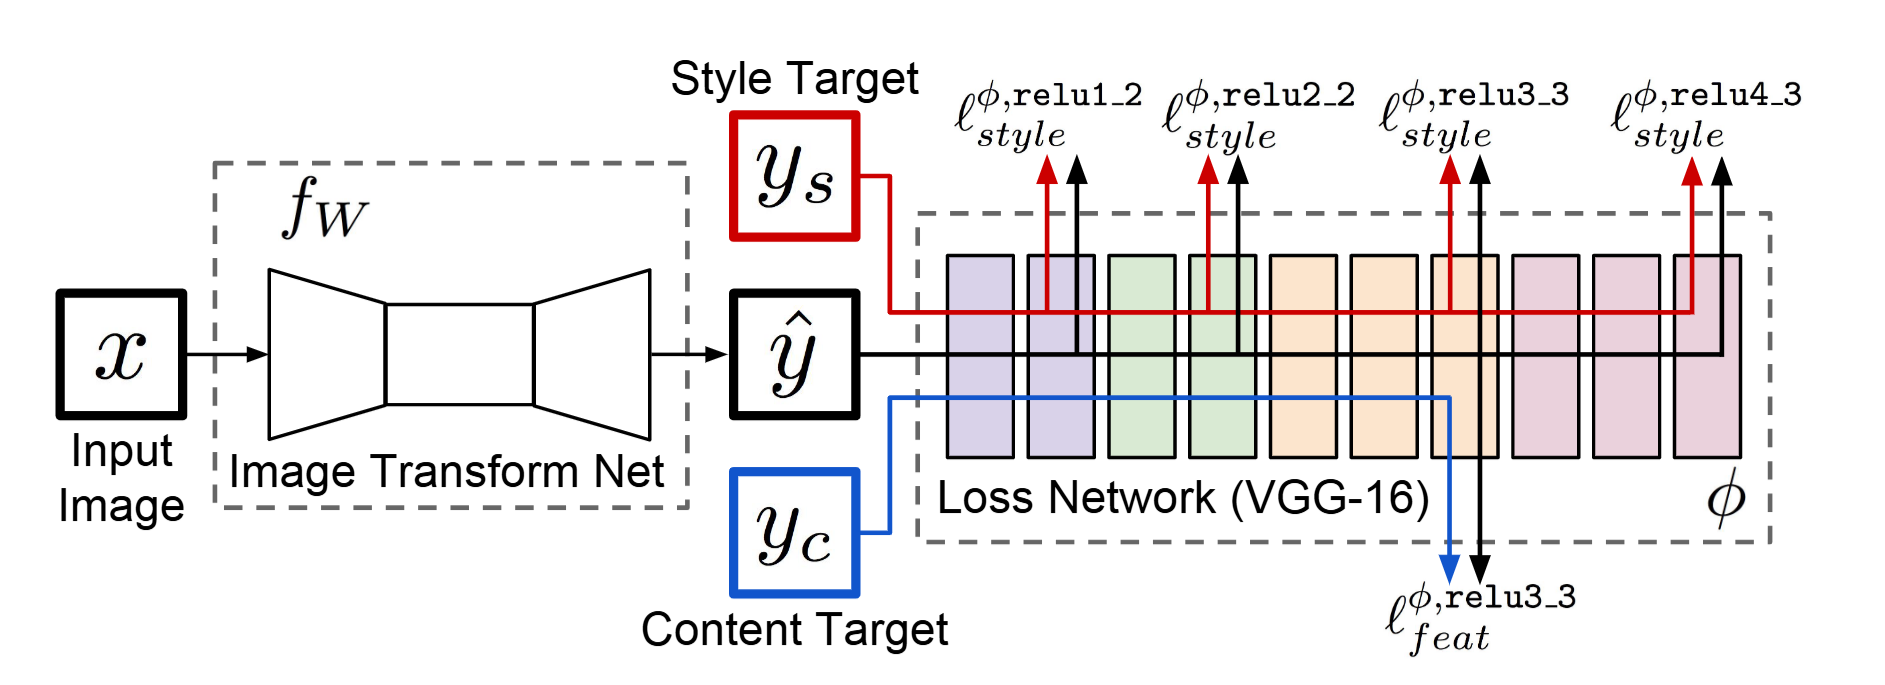
\includegraphics[width=0.9\textwidth]{img/1.png}
\caption{网络的基本结构,摘自 \cite{johnson2016perceptual}。}
\label{fig:network}
\end{figure}

\subsubsection{感知损失与 VGG 网络}

为度量图像的内容与风格差异,该方法引入一个在 ImageNet\cite{deng2009imagenet} 上预训练的 VGG-16 网络\cite{simonyan2014very} $\phi$作为固定的损失网络,从中提取图像的中高层语义特征。损失函数由三部分组成:

\begin{enumerate}
    \item[1)] \textbf{内容损失(Content Loss)}
    
    内容损失衡量输出图像 $\hat{y}$ 与内容图像 $y_c$ 在 VGG 网络中某一中间层 $j$ 的特征表示之间的差异:

    \begin{equation}
    \mathcal{L}_{\text{content}}(\hat{y}, y_c) = \frac{1}{C_j H_j W_j} \left\| \phi_j(\hat{y}) - \phi_j(y_c) \right\|_2^2
    \end{equation}

    其中,$\phi_j(x)$ 表示图像 $x$ 在第 $j$ 层的特征图,$C_j, H_j, W_j$ 分别为通道数、高度和宽度。

\item[2)] \textbf{风格损失(Style Loss)}  

风格损失基于多个卷积层提取的特征图的 Gram 矩阵,可以衡量输出图像 $\hat{y}$ 与风格图像 $y_s$ 在纹理上的相似性:

\begin{equation}
G_j(x) = \frac{1}{C_j H_j W_j} \phi_j(x) \phi_j(x)^T
\end{equation}

\begin{equation}
\mathcal{L}_{\text{style}}(\hat{y}, y_s) = \sum_{j \in \mathcal{S}} \left\| G_j(\hat{y}) - G_j(y_s) \right\|_F^2
\end{equation}

其中 $\mathcal{S}$ 为选定的风格层集合(如 \texttt{relu1\_2}, \texttt{relu2\_2}, \texttt{relu3\_3}, \texttt{relu4\_3})。

\item[3)] \textbf{总变差正则项(Total Variation Regularization)} 

总变差正则项用于鼓励输出图像在空间上具有平滑性,它可以抑制噪声和伪影。

\begin{equation}
\mathcal{L}_{\text{TV}}(\hat{y}) = \sum_{i,j} \left( (\hat{y}_{i,j+1} - \hat{y}_{i,j})^2 + (\hat{y}_{i+1,j} - \hat{y}_{i,j})^2 \right)
\end{equation}
\end{enumerate}


\subsubsection{训练目标}

综合上述损失项,图像变换网络的训练目标函数为:

\begin{equation}
\min_W \ \mathbb{E}_{x \sim \mathcal{D}} \left[ \lambda_c \mathcal{L}_{\text{content}}(f_W(x), y_c) + \lambda_s \mathcal{L}_{\text{style}}(f_W(x), y_s) + \lambda_{TV} \mathcal{L}_{\text{TV}}(f_W(x)) \right]
\end{equation}

其中 $\lambda_c, \lambda_s, \lambda_{TV}$ 为各损失项的权重系数,$\mathcal{D}$ 表示训练图像集。


\newpage
\subsection{所选神经网络模型亮点}

\begin{enumerate}[noitemsep]
    \item[1)] 该模型使用基于深度卷积网络的特征空间差异作为损失函数,而不是简单的像素级 MSE。这样能更好捕捉图像的高层语义和纹理信息,使得风格迁移结果更自然、更艺术化;
    \item[2)] 该模型设计了一个轻量级的前馈卷积网络,训练时用感知损失约束风格和内容,推理时只需一次前向传播即可生成风格化图像,速度远快于传统基于优化的风格迁移方法,相比 \cite{gatys2015neural},速度提升了数百倍甚至上千倍;
    \item[3)] 该模型训练时间短,通常只需数小时即可完成训练,便于完成实验。 
\end{enumerate}

\section{实验过程}

\subsection{实验环境}

本次实验在以下环境下进行:

\begin{itemize}[noitemsep]
    \item 操作系统:Windows 11 家庭中文版 26100.4061
    \item 显卡:NVIDIA RTX 3070 Laptop
    \item 深度学习框架:PyTorch 2.7.0+cu126
\end{itemize}

\subsection{实验步骤}

\begin{enumerate}[noitemsep]
    \item 下载数据集:本实验使用了 ImageNet \cite{deng2009imagenet} 数据集的一个子集,共包含 50000 张图像;
    \item 下载预训练模型:使用 VGG-16 网络作为损失网络,下载预训练模型并加载;
    \item 训练图像变换网络:使用训练集对图像变换网络进行训练,设置超参数;
    \item 生成风格化图像:使用训练好的图像变换网络对测试图像进行风格迁移,生成风格化图像;
\end{enumerate}

\section{实验结果与分析}

\begin{figure}[H]
\centering
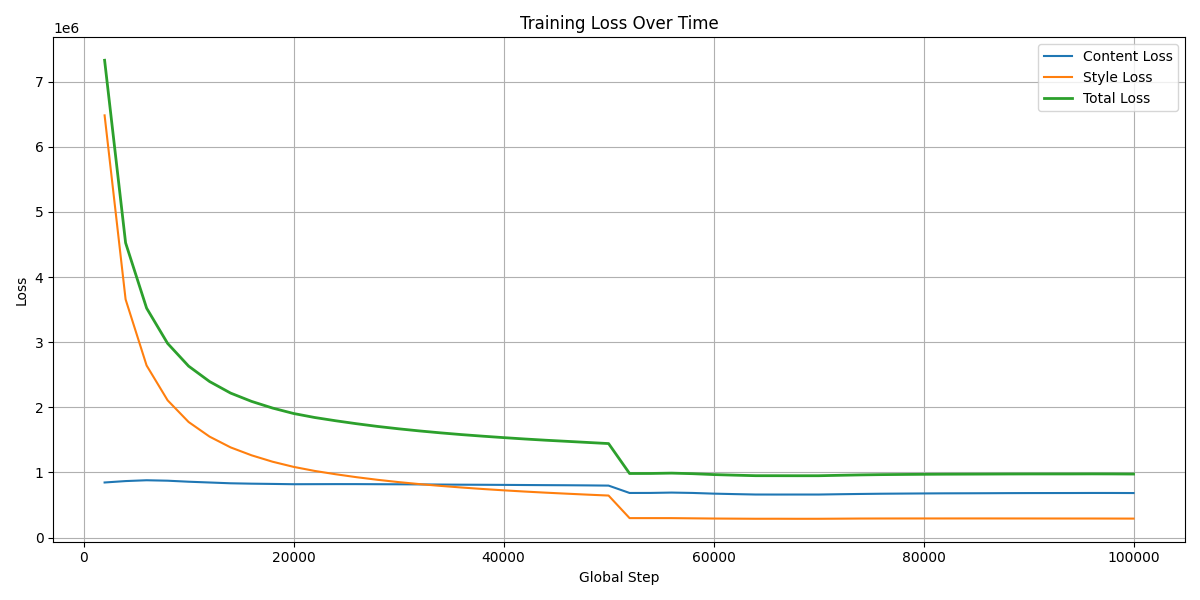
\includegraphics[width=0.7\textwidth]{img/loss_1.png}
\caption{训练过程中损失函数的变化曲线}
\label{fig:loss}
\end{figure}

图 \ref{fig:loss} 展示了训练过程中损失函数的变化曲线。可以看到,随着训练的进行,内容损失和风格损失逐渐减小,总损失也趋于平稳,表明模型在不断学习和优化。最终,模型的总Loss收敛在 $0.9 \times 10^6$ 左右。

当前 20000 次迭代时,内容损失和风格损失的变化较大,说明模型在学习初期对内容和风格特征的提取能力较弱。随着迭代次数的增加,损失函数逐渐收敛,表明模型对内容和风格特征的提取能力逐渐增强。而最后 60000 次迭代时,损失函数的变化幅度较小,说明模型已经趋于收敛,内容和风格特征的提取能力达到了较高水平。

\begin{figure}[H]
\centering
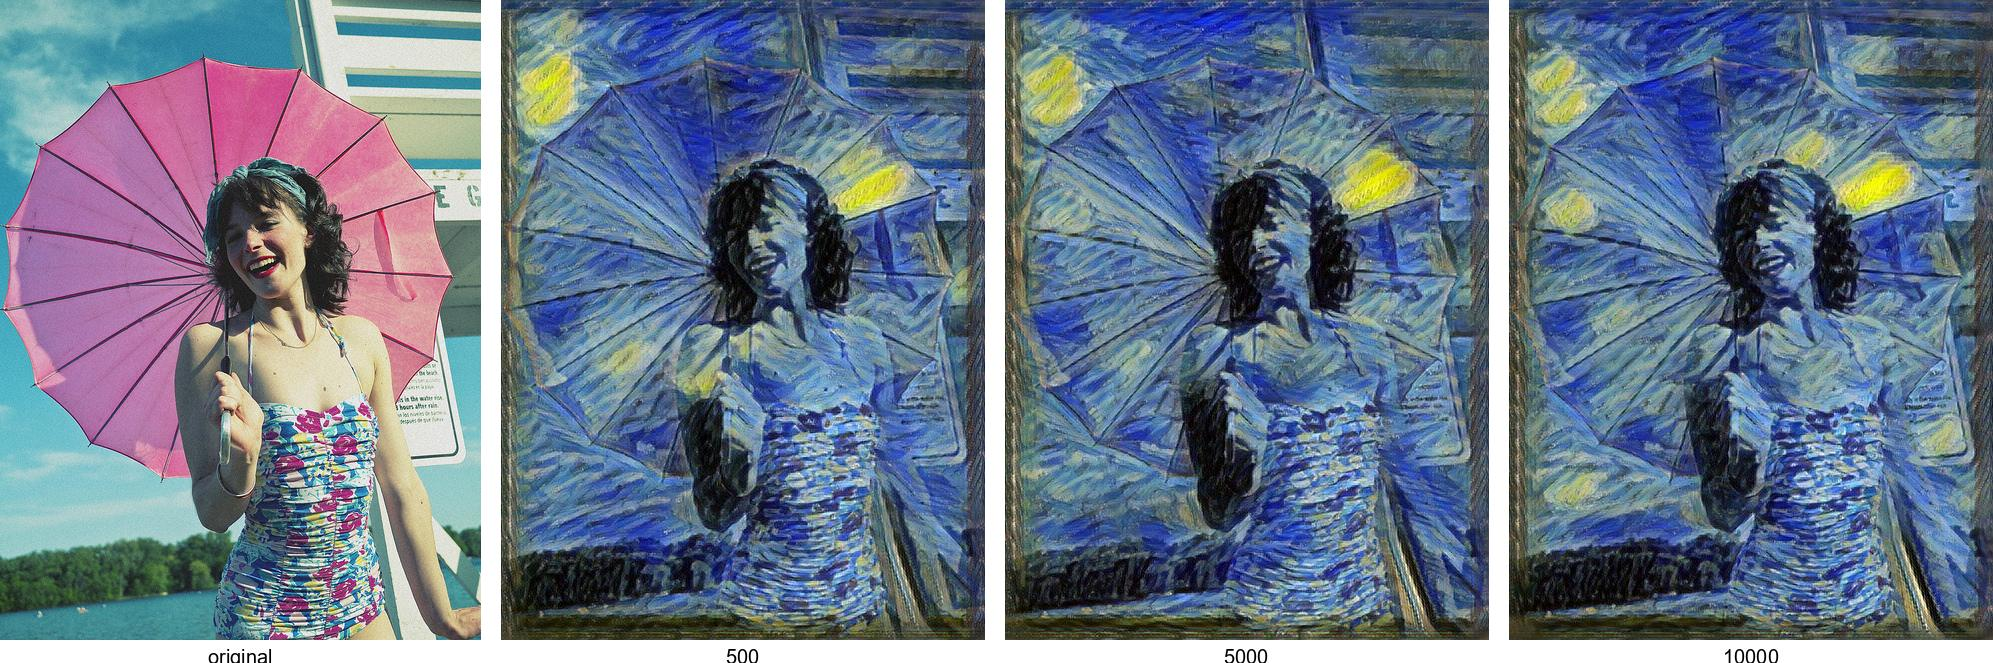
\includegraphics[width=0.8\textwidth]{img/output.jpg}
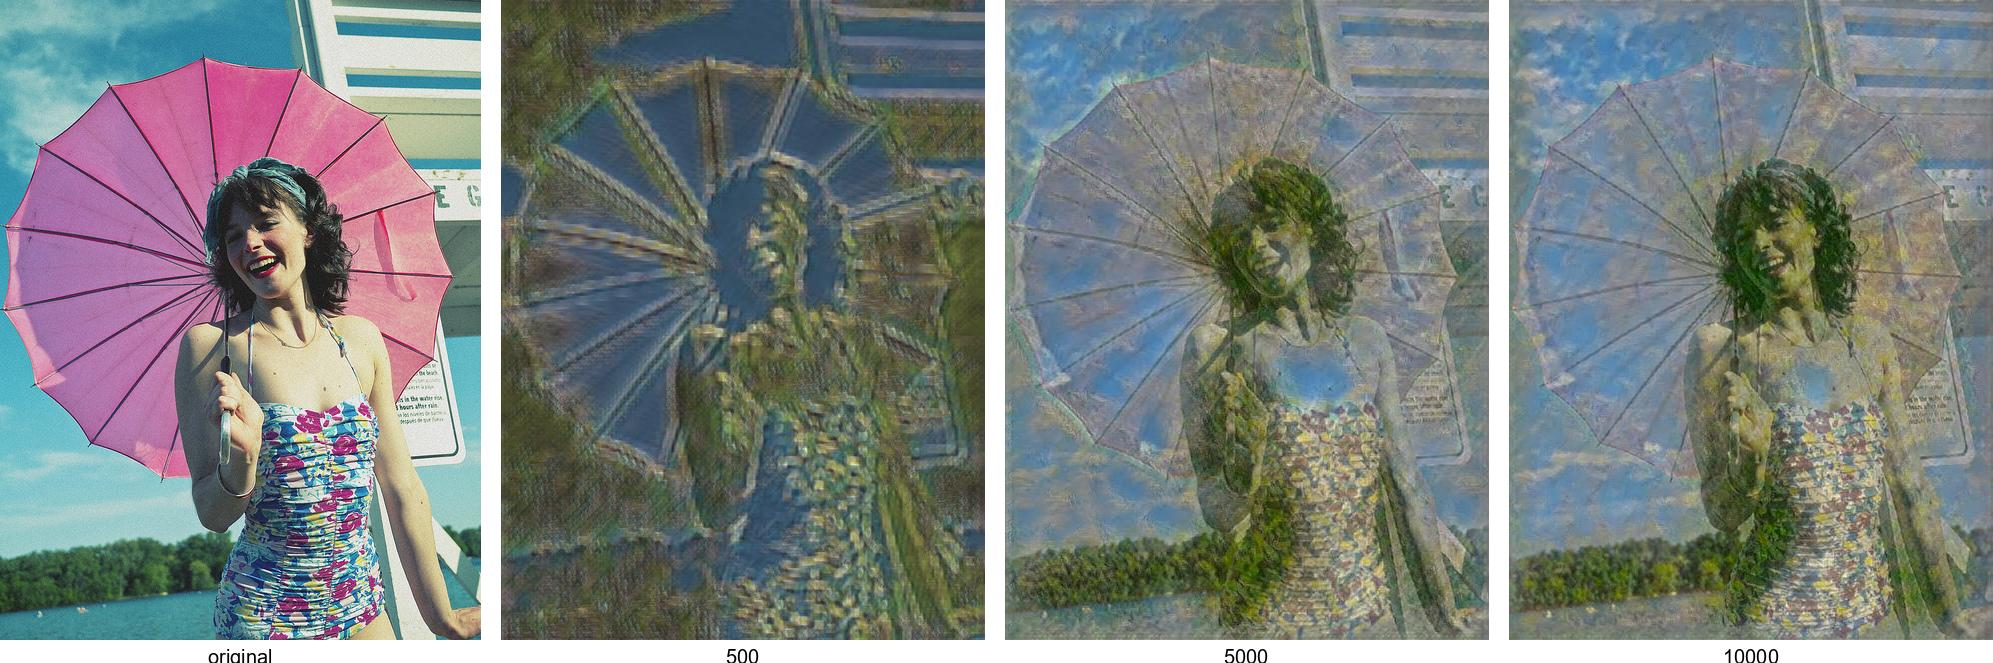
\includegraphics[width=0.8\textwidth]{img/output2.jpg}
\caption{不同迭代次数下的风格迁移结果,风格分别为《星月夜》和《撑阳伞的女人》}
\label{fig:output}
\end{figure}

图 \ref{fig:output} 展示了不同迭代次数下的风格迁移结果。可以看到,随着迭代次数的增加,生成的风格化图像质量逐渐提高,细节更加丰富,纹理更加自然。

风格迁移所用时间在0.05秒左右。

\section{实验总结}

本次实验实现了基于深度学习的图像风格迁移方法,使用了 Fast Style Transfer 模型。通过对模型的训练和测试,验证了该方法在风格迁移任务中的有效性和高效性。


\newpage
\phantomsection
\addcontentsline{toc}{section}{参考文献}
\printbibliography[title={\zihao{-3} \heiti \centering 参\ 考\ 文\ 献}]


\end{document}

